% This contents of this file will be inserted into the _Solutions version of the
% output tex document.  Here's an example:

% If assignment with subquestion (1.a) requires a written response, you will
% find the following flag within this document: <SCPD_SUBMISSION_TAG>_1a
% In this example, you would insert the LaTeX for your solution to (1.a) between
% the <SCPD_SUBMISSION_TAG>_1a flags.  If you also constrain your answer between the
% START_CODE_HERE and END_CODE_HERE flags, your LaTeX will be styled as a
% solution within the final document.

% Please do not use the '<SCPD_SUBMISSION_TAG>' character anywhere within your code.  As expected,
% that will confuse the regular expressions we use to identify your solution.
\def\assignmentnum{3 }
\def\assignmenttitle{XCS330 Problem Set \assignmentnum}

\documentclass{article}
\usepackage[top = 1.0in]{geometry}

\usepackage{graphicx}

\usepackage[utf8]{inputenc}
\usepackage{listings}
\usepackage[dvipsnames]{xcolor}
\usepackage{bm}
\usepackage{algorithm}
\usepackage{algpseudocode}
\usepackage{framed}
\usepackage{xspace}

\definecolor{codegreen}{rgb}{0,0.6,0}
\definecolor{codegray}{rgb}{0.5,0.5,0.5}
\definecolor{codepurple}{rgb}{0.58,0,0.82}
\definecolor{backcolour}{rgb}{0.95,0.95,0.92}

\lstdefinestyle{mystyle}{
    backgroundcolor=\color{backcolour},   
    commentstyle=\color{codegreen},
    keywordstyle=\color{magenta},
    stringstyle=\color{codepurple},
    basicstyle=\ttfamily\footnotesize,
    breakatwhitespace=false,         
    breaklines=true,                 
    captionpos=b,                    
    keepspaces=true,                 
    numbersep=5pt,                  
    showspaces=false,                
    showstringspaces=false,
    showtabs=false,                  
    tabsize=2
}

\lstset{style=mystyle}

\newcommand{\di}{{d}}
\newcommand{\nexp}{{n}}
\newcommand{\nf}{{p}}
\newcommand{\vcd}{{\textbf{D}}}
\newcommand{\Int}{\mathbb{Z}}
\newcommand\bb{\ensuremath{\mathbf{b}}}
\newcommand\bs{\ensuremath{\mathbf{s}}}
\newcommand\bp{\ensuremath{\mathbf{p}}}
\newcommand{\relu} { \operatorname{ReLU} }
\newcommand{\smx} { \operatorname{softmax} }
\newcommand\bx{\ensuremath{\mathbf{x}}}
\newcommand\bh{\ensuremath{\mathbf{h}}}
\newcommand\bc{\ensuremath{\mathbf{c}}}
\newcommand\bW{\ensuremath{\mathbf{W}}}
\newcommand\by{\ensuremath{\mathbf{y}}}
\newcommand\bo{\ensuremath{\mathbf{o}}}
\newcommand\be{\ensuremath{\mathbf{e}}}
\newcommand\ba{\ensuremath{\mathbf{a}}}
\newcommand\bu{\ensuremath{\mathbf{u}}}
\newcommand\bv{\ensuremath{\mathbf{v}}}
\newcommand\bP{\ensuremath{\mathbf{P}}}
\newcommand\bg{\ensuremath{\mathbf{g}}}
\newcommand\bX{\ensuremath{\mathbf{X}}}
% real numbers R symbol
\newcommand{\Real}{\mathbb{R}}

% encoder hidden
\newcommand{\henc}{\bh^{\text{enc}}}
\newcommand{\hencfw}[1]{\overrightarrow{\henc_{#1}}}
\newcommand{\hencbw}[1]{\overleftarrow{\henc_{#1}}}

% encoder cell
\newcommand{\cenc}{\bc^{\text{enc}}}
\newcommand{\cencfw}[1]{\overrightarrow{\cenc_{#1}}}
\newcommand{\cencbw}[1]{\overleftarrow{\cenc_{#1}}}

% decoder hidden
\newcommand{\hdec}{\bh^{\text{dec}}}

% decoder cell
\newcommand{\cdec}{\bc^{\text{dec}}}

\usepackage[hyperfootnotes=false]{hyperref}
\hypersetup{
  colorlinks=true,
  linkcolor = blue,
  urlcolor  = blue,
  citecolor = blue,
  anchorcolor = blue,
  pdfborderstyle={/S/U/W 1}
}
\usepackage{nccmath}
\usepackage{mathtools}
\usepackage{graphicx,caption}
\usepackage[shortlabels]{enumitem}
\usepackage{epstopdf,subcaption}
\usepackage{psfrag}
\usepackage{amsmath,amssymb,epsf}
\usepackage{verbatim}
\usepackage{cancel}
\usepackage{color,soul}
\usepackage{bbm}
\usepackage{listings}
\usepackage{setspace}
\usepackage{float}
\definecolor{Code}{rgb}{0,0,0}
\definecolor{Decorators}{rgb}{0.5,0.5,0.5}
\definecolor{Numbers}{rgb}{0.5,0,0}
\definecolor{MatchingBrackets}{rgb}{0.25,0.5,0.5}
\definecolor{Keywords}{rgb}{0,0,1}
\definecolor{self}{rgb}{0,0,0}
\definecolor{Strings}{rgb}{0,0.63,0}
\definecolor{Comments}{rgb}{0,0.63,1}
\definecolor{Backquotes}{rgb}{0,0,0}
\definecolor{Classname}{rgb}{0,0,0}
\definecolor{FunctionName}{rgb}{0,0,0}
\definecolor{Operators}{rgb}{0,0,0}
\definecolor{Background}{rgb}{0.98,0.98,0.98}
\lstdefinelanguage{Python}{
    numbers=left,
    numberstyle=\footnotesize,
    numbersep=1em,
    xleftmargin=1em,
    framextopmargin=2em,
    framexbottommargin=2em,
    showspaces=false,
    showtabs=false,
    showstringspaces=false,
    frame=l,
    tabsize=4,
    % Basic
    basicstyle=\ttfamily\footnotesize\setstretch{1},
    backgroundcolor=\color{Background},
    % Comments
    commentstyle=\color{Comments}\slshape,
    % Strings
    stringstyle=\color{Strings},
    morecomment=[s][\color{Strings}]{"""}{"""},
    morecomment=[s][\color{Strings}]{'''}{'''},
    % keywords
    morekeywords={import,from,class,def,for,while,if,is,in,elif,else,not,and,or
    ,print,break,continue,return,True,False,None,access,as,,del,except,exec
    ,finally,global,import,lambda,pass,print,raise,try,assert},
    keywordstyle={\color{Keywords}\bfseries},
    % additional keywords
    morekeywords={[2]@invariant},
    keywordstyle={[2]\color{Decorators}\slshape},
    emph={self},
    emphstyle={\color{self}\slshape},
%
}
\lstMakeShortInline|

\pagestyle{empty} \addtolength{\textwidth}{1.0in}
\addtolength{\textheight}{0.5in}
\addtolength{\oddsidemargin}{-0.5in}
\addtolength{\evensidemargin}{-0.5in}
\newcommand{\ruleskip}{\bigskip\hrule\bigskip}
\newcommand{\nodify}[1]{{\sc #1}}
\newenvironment{answer}{\sf \begingroup\color{ForestGreen}}{\endgroup}%

\setlist[itemize]{itemsep=2pt, topsep=0pt}
\setlist[enumerate]{itemsep=6pt, topsep=0pt}

\setlength{\parindent}{0pt}
\setlength{\parskip}{4pt}
\setlist[enumerate]{parsep=4pt}
\setlength{\unitlength}{1cm}

\renewcommand{\Re}{{\mathbb R}}
\newcommand{\R}{\mathbb{R}}
\newcommand{\what}[1]{\widehat{#1}}

\renewcommand{\comment}[1]{}
\newcommand{\mc}[1]{\mathcal{#1}}
\newcommand{\half}{\frac{1}{2}}

\DeclareMathOperator*{\argmin}{arg\,min}

\def\KL{D_{KL}}
\def\xsi{x^{(i)}}
\def\ysi{y^{(i)}}
\def\zsi{z^{(i)}}
\def\E{\mathbb{E}}
\def\calN{\mathcal{N}}
\def\calD{\mathcal{D}}
\def\slack{\url{http://xcs224n-scpd.slack.com/}}
\def\zipscriptalt{\texttt{python zip\_submission.py}}
\DeclarePairedDelimiter\abs{\lvert}{\rvert}%
 
\usepackage{bbding}
\usepackage{pifont}
\usepackage{wasysym}
\usepackage{amssymb}
\usepackage{framed}
\usepackage{scrextend}

\newcommand{\alns}[1] {
	\begin{align*} #1 \end{align*}
}

\newcommand{\pd}[2] {
 \frac{\partial #1}{\partial #2}
}
\renewcommand{\Re} { \mathbb{R} }
\newcommand{\btx} { \mathbf{\tilde{x}} }
\newcommand{\bth} { \mathbf{\tilde{h}} }
\newcommand{\sigmoid} { \operatorname{\sigma} }
\newcommand{\CE} { \operatorname{CE} }
\newcommand{\byt} { \hat{\by} }
\newcommand{\yt} { \hat{y} }

\newcommand{\oft}[1]{^{(#1)}}
\newcommand{\fone}{\ensuremath{F_1}}

\newcommand{\ac}[1]{ {\color{red} \textbf{AC:} #1} }
\newcommand{\ner}[1]{\textbf{\color{blue} #1}}

\begin{document}
\pagestyle{myheadings} \markboth{}{\assignmenttitle}

% <SCPD_SUBMISSION_TAG>_entire_submission

This handout includes space for every question that requires a written response.
Please feel free to use it to handwrite your solutions (legibly, please).  If
you choose to typeset your solutions, the |README.md| for this assignment includes
instructions to regenerate this handout with your typeset \LaTeX{} solutions.
\ruleskip

\LARGE
1.a
\normalsize

% <SCPD_SUBMISSION_TAG>_1_a
\begin{answer}
    % ### START CODE HERE ###
    In the previous homework recall that we used an LSTM model and that we needed to shuffle the query set so that the model didn't learn to output the same sequence of classes without learning to recognize the images.\\ 
	For protonets a mapping function is learned that places images of the same class close to each other in feature space. 
	For each class a prototype is calculated. The mapping function is used on the query example placing it in the feature space. 
	Then using a distance function the query example is placed into the class who's class prototype is closest to it. 
	Since then operations of mapping the image into feature space and calculating the distance of the example to the prototype do not use the order of the queries, shuffling the queries is not needed. 
    % ### END CODE HERE ###
\end{answer}
% <SCPD_SUBMISSION_TAG>_1_a

\clearpage

\LARGE
1.c.i
\normalsize

% <SCPD_SUBMISSION_TAG>_1_c_i
\begin{answer}
    % ### START CODE HERE ###
	\begin{center}
		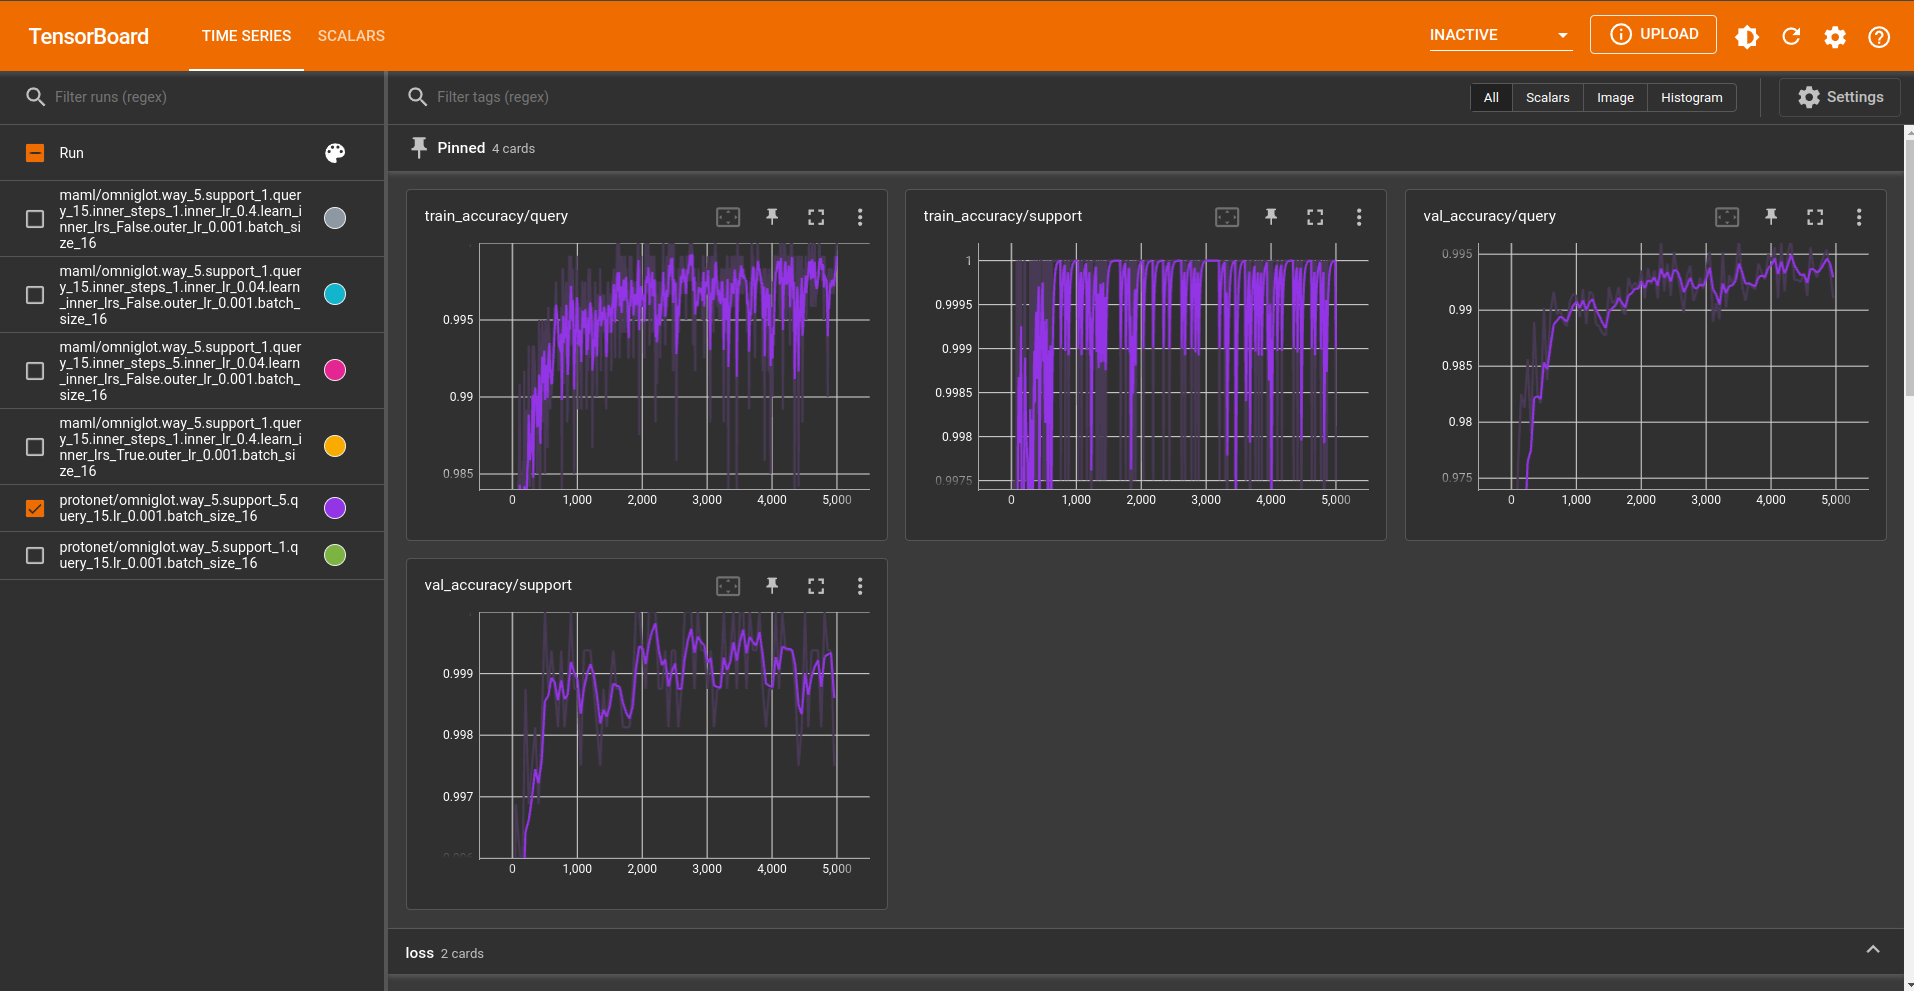
\includegraphics[width=1.0\textwidth]{proto_5_5}
	\end{center}
	Looking at the graphs above we can see that the train accuracy and validation accuracy for the support classes are around 99\%. 
	This indicates that the examples from the same class are being placed close together in feature space.
    % ### END CODE HERE ###
\end{answer}
% <SCPD_SUBMISSION_TAG>_1_c_i

\LARGE
1.c.ii
\normalsize

% <SCPD_SUBMISSION_TAG>_1_c_ii
\begin{answer}
    % ### START CODE HERE ###
	Looking at the graphs in 1.c.i it seems that the model is generalizing to new tasks as the validation accuracy for the query and support is around 99\%. 
    % ### END CODE HERE ###
\end{answer}
% <SCPD_SUBMISSION_TAG>_1_c_ii

\clearpage

\LARGE
1.d.i
\normalsize

% <SCPD_SUBMISSION_TAG>_1_d_i
\begin{answer}
    % ### START CODE HERE ###
	\begin{center}
		\begin{tabular}{c c c}
		        \hline
			 & 5 way 5 support & 5 way 1 support \\
			\hline
			Mean & 0.972 & 0.98 \\
			\hline
			95\% Confidence Interval & 0.003 & 0.002 \\
			\hline
		\end{tabular}
	\end{center}
    % ### END CODE HERE ###
\end{answer}
% <SCPD_SUBMISSION_TAG>_1_d_i

\LARGE
1.d.ii
\normalsize

% <SCPD_SUBMISSION_TAG>_1_d_ii
\begin{answer}
    % ### START CODE HERE ###
	The checkpoint of 4900 was chosen because it was the latest checkpoint.
    % ### END CODE HERE ###
\end{answer}
% <SCPD_SUBMISSION_TAG>_1_d_ii

\LARGE
1.d.iii
\normalsize

% <SCPD_SUBMISSION_TAG>_1_d_iii
\begin{answer}
    % ### START CODE HERE ###
	No there was not a significant difference between 5 shot and 1 shot performance. \\
	To explain why we need to look at what the support features are being used for. \\
	The support features are used for calculating the class prototype which is the mean of the support features. \\
	With a shot of 1 the mean of the support features is the one support feature itself and if it accurately represents the underlying class is as good as the class prototype produced with a higher shot. \\
	What you get with a higher shot is that the class prototype is more likely to represent the underlying class' distribution accurately. \\
    % ### END CODE HERE ###
\end{answer}
% <SCPD_SUBMISSION_TAG>_1_d_iii
        
\clearpage

\LARGE
2.c.i
\normalsize

% <SCPD_SUBMISSION_TAG>_2_c_i
\begin{answer}
    % ### START CODE HERE ###
	\begin{center}
		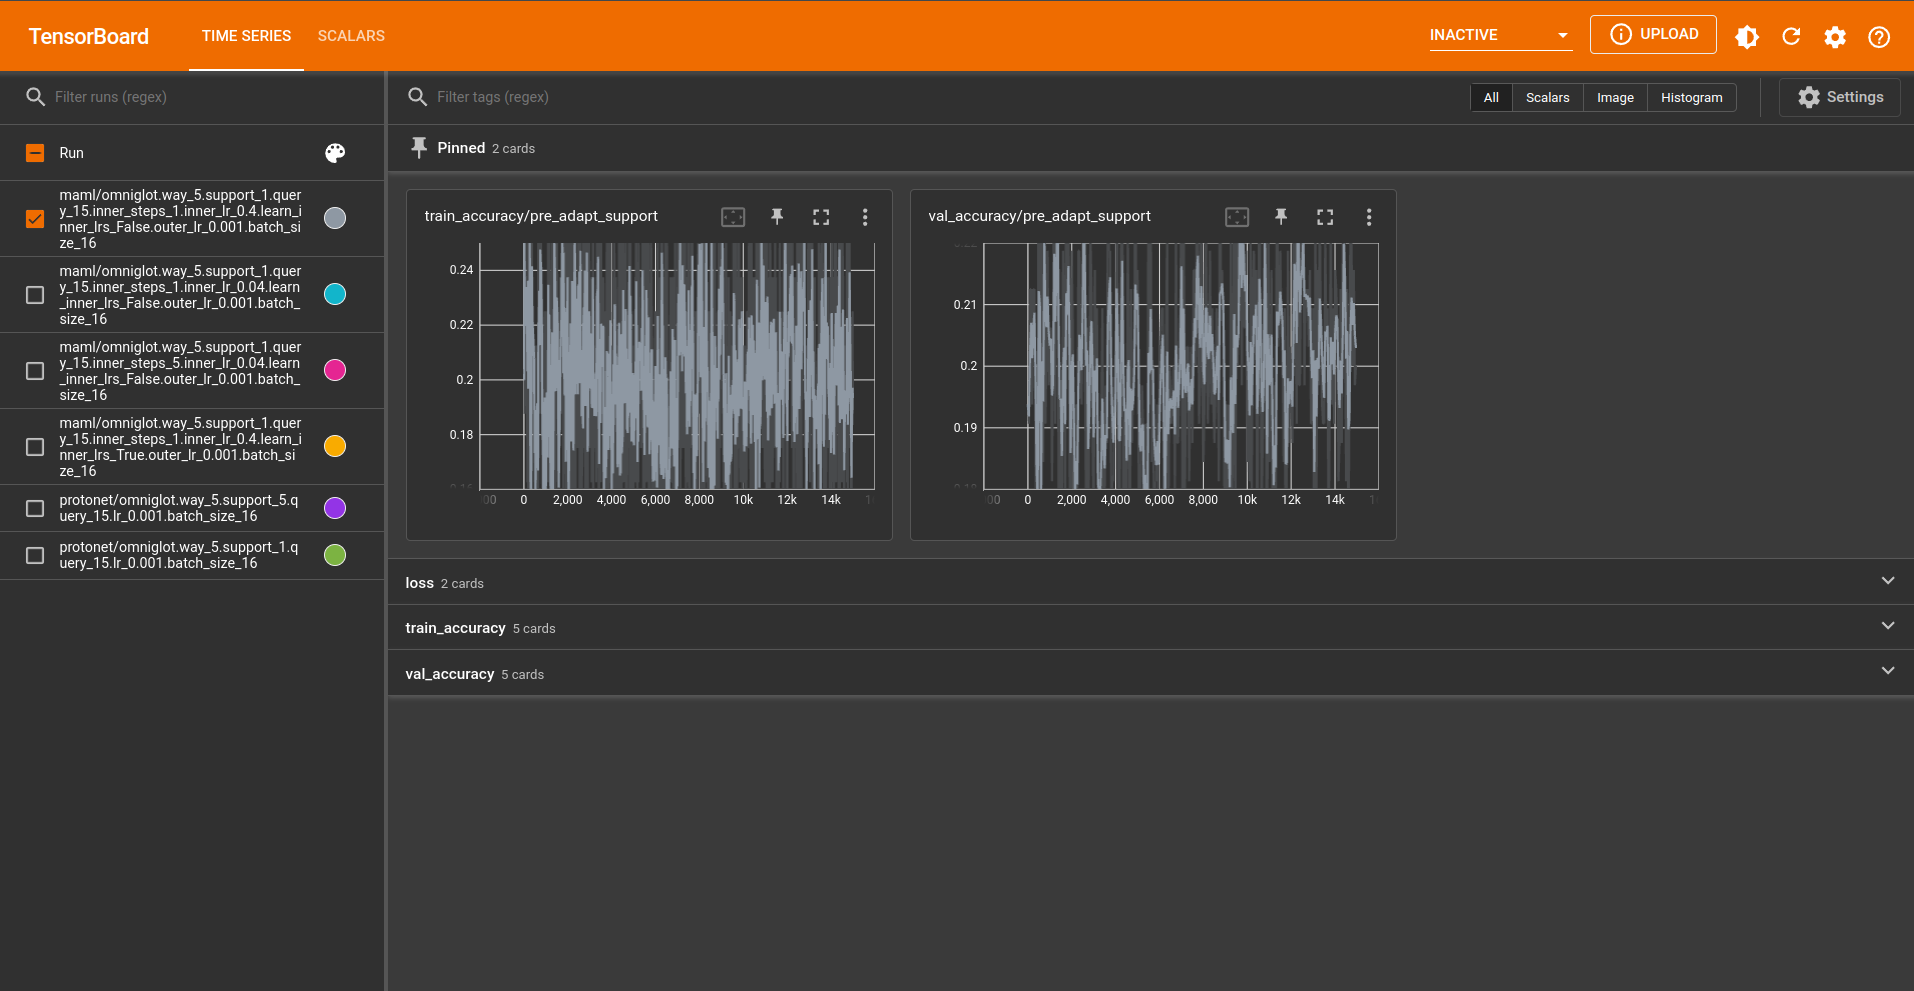
\includegraphics[width=1.0\textwidth]{pre_adapt}
	\end{center}
	The train and validation accuracy is poor. \\
	This is because the adaptations for each task has not occured yet. \\
	The model is fit to all tasks.
    % ### END CODE HERE ###
\end{answer}
% <SCPD_SUBMISSION_TAG>_2_c_i

\LARGE
2.c.ii
\normalsize

% <SCPD_SUBMISSION_TAG>_2_c_ii
\begin{answer}
    % ### START CODE HERE ###
	\begin{center}
		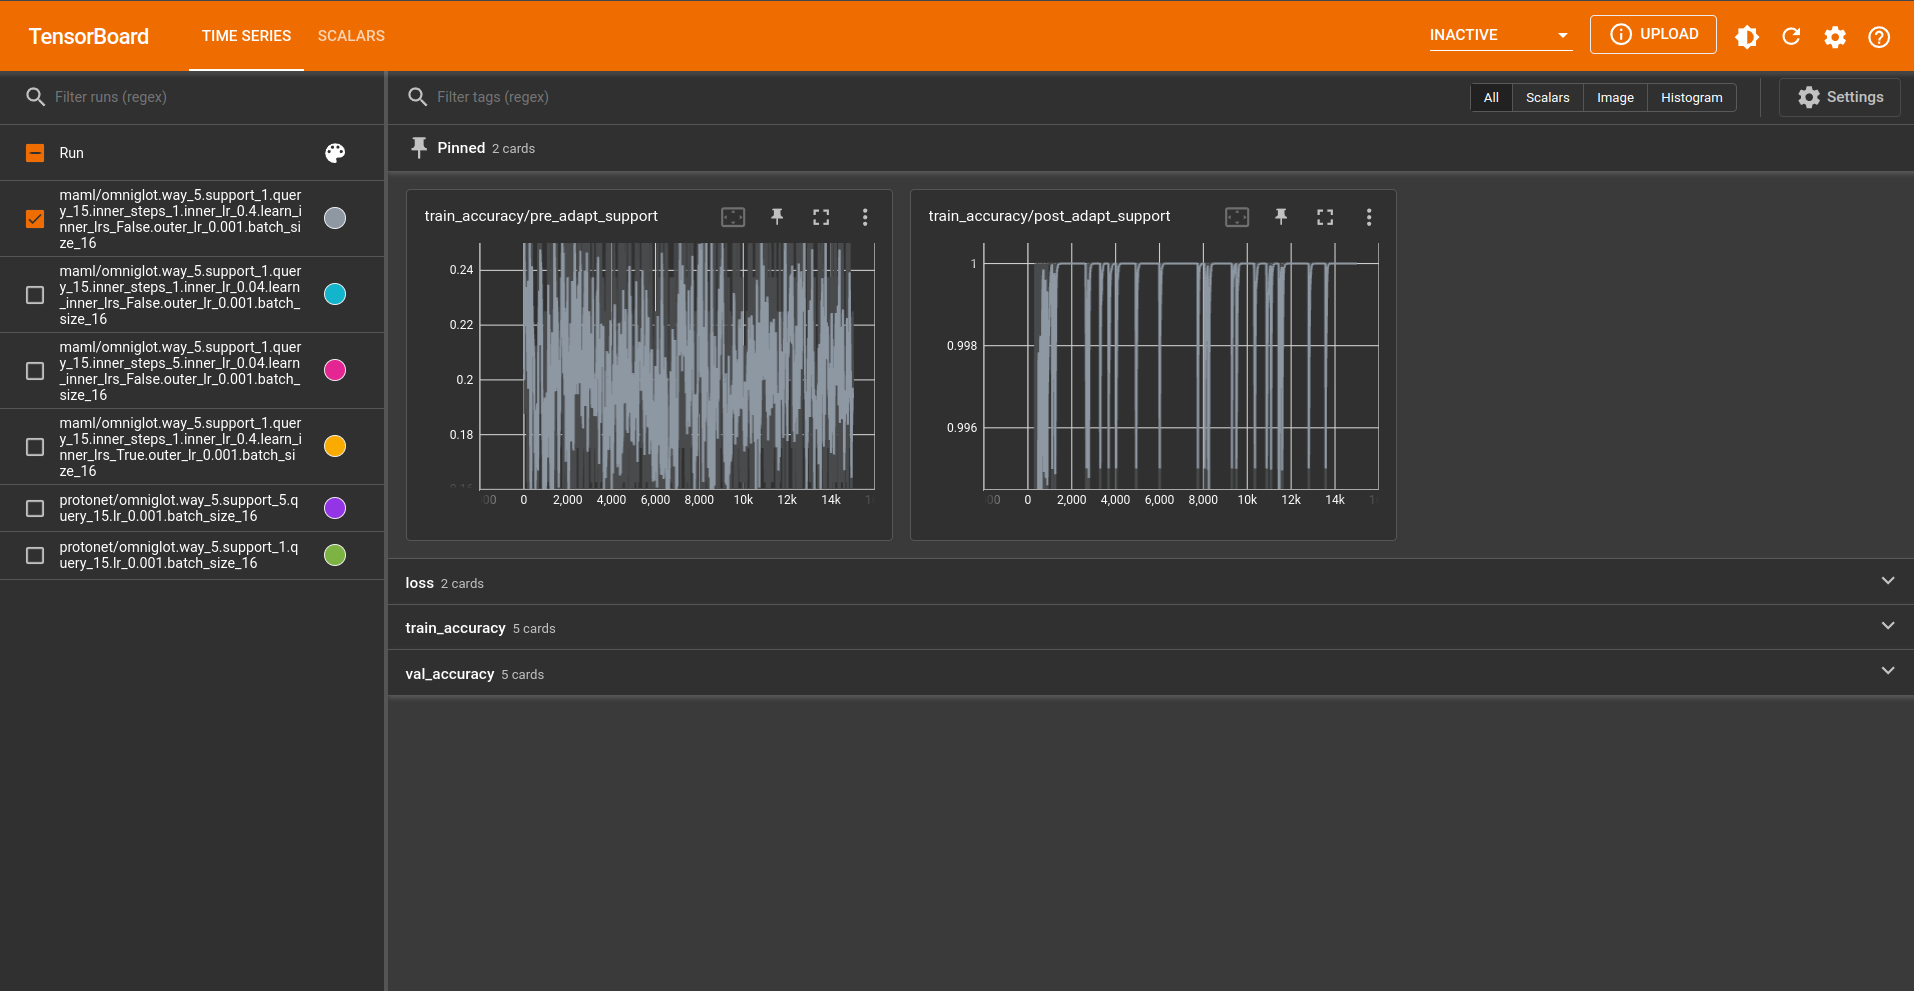
\includegraphics[width=1.0\textwidth]{pre_post_adapt_support}
	\end{center}
	The post adapt support accuracy is much better than the pre adapt support accuracy. \\
	This tells us that the model is not good at any of the particular tasks on it's own without adaptation.
    % ### END CODE HERE ###
\end{answer}
% <SCPD_SUBMISSION_TAG>_2_c_ii

\LARGE
2.c.iii
\normalsize

% <SCPD_SUBMISSION_TAG>_2_c_iii
\begin{answer}
    % ### START CODE HERE ###
	\begin{center}
		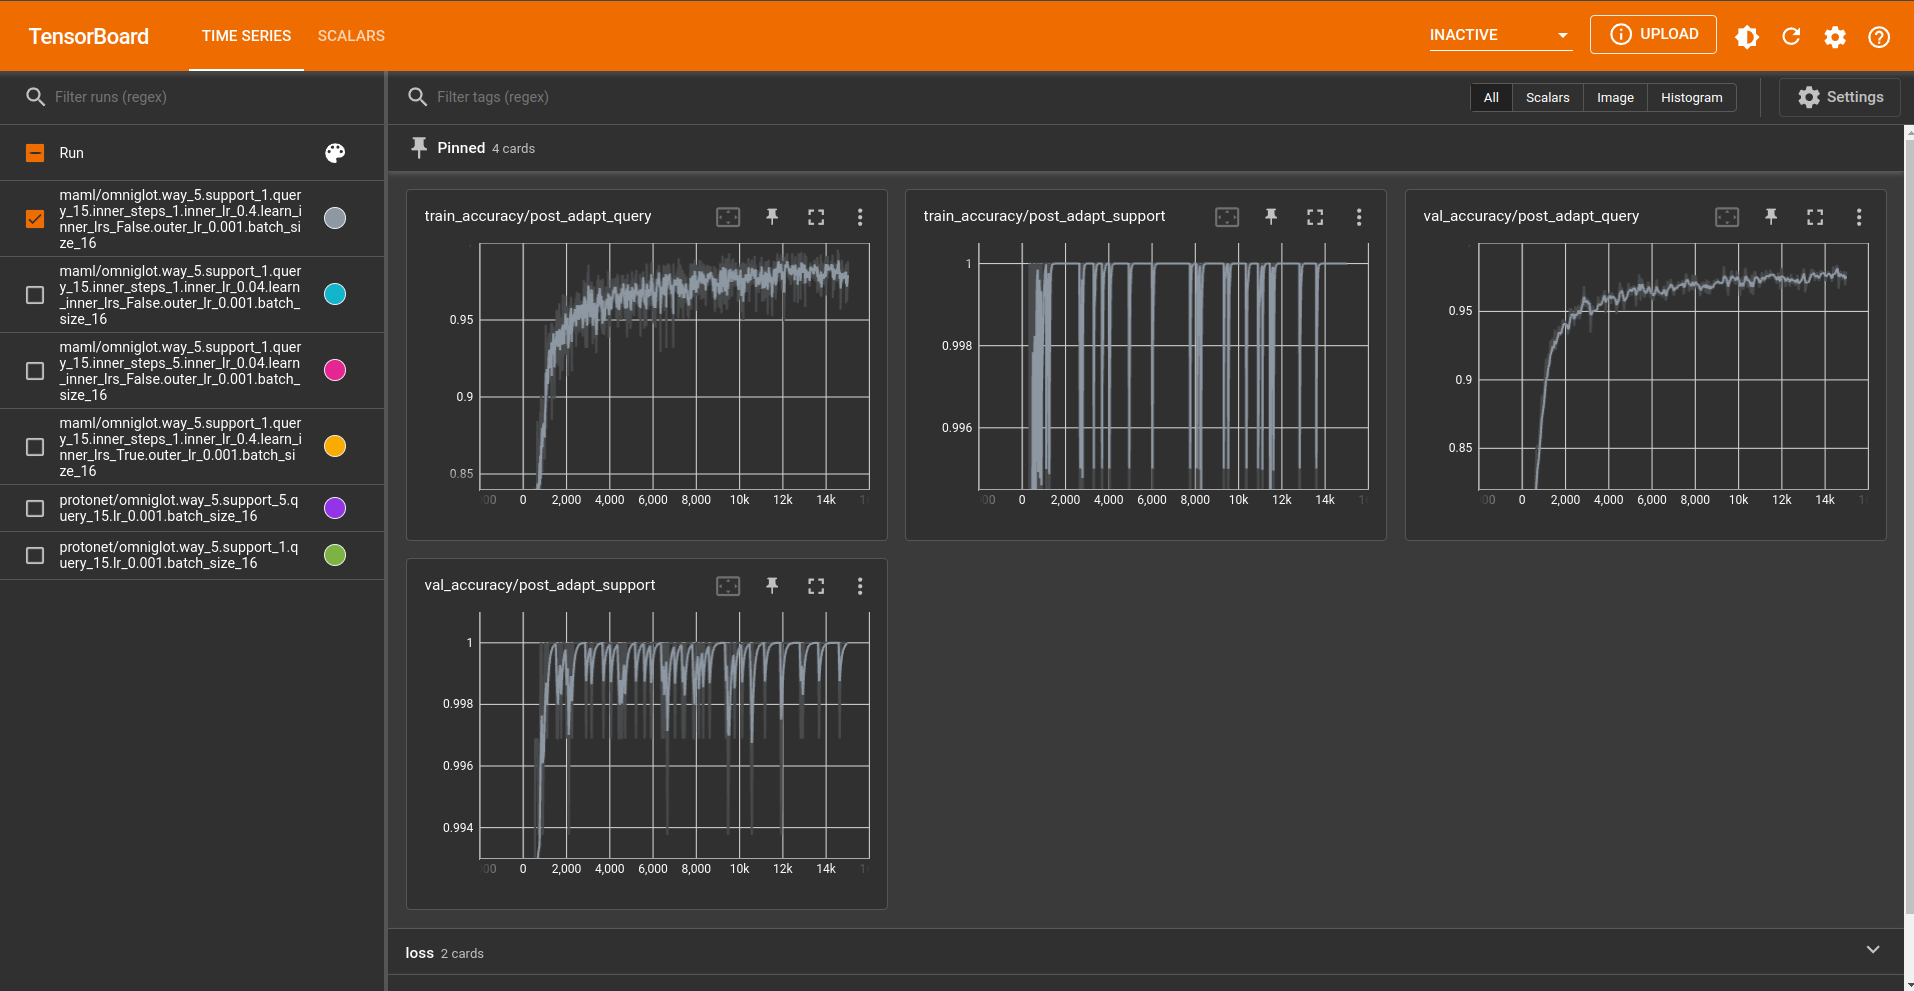
\includegraphics[width=1.0\textwidth]{post}
	\end{center}
	Both the post train adapt query and train post support accuracies are good with greater than 95\% accuracy. \\
	This tells us that the adaptation is working and generalizing to new cases of the tasks. \\
	Both the post validation adapt query and support accuracies are good with greater than 95\% accuracy. \\
	This tells us that the adaptation is working and generalizing to new cases of the tasks.
    % ### END CODE HERE ###
\end{answer}
% <SCPD_SUBMISSION_TAG>_2_c_iii

\clearpage

\LARGE
2.d.i
\normalsize

% <SCPD_SUBMISSION_TAG>_2_d_i
\begin{answer}
    % ### START CODE HERE ###
	\begin{center}
		\includegraphics[width=1.0\textwidth]{lr\_diff}
	\end{center}
	Lowering the learning rate makes the model learn slower. 
    % ### END CODE HERE ###
\end{answer}
% <SCPD_SUBMISSION_TAG>_2_d_i


\LARGE
2.d.ii
\normalsize

% <SCPD_SUBMISSION_TAG>_2_d_ii
\begin{answer}
    % ### START CODE HERE ###
	\begin{center}
		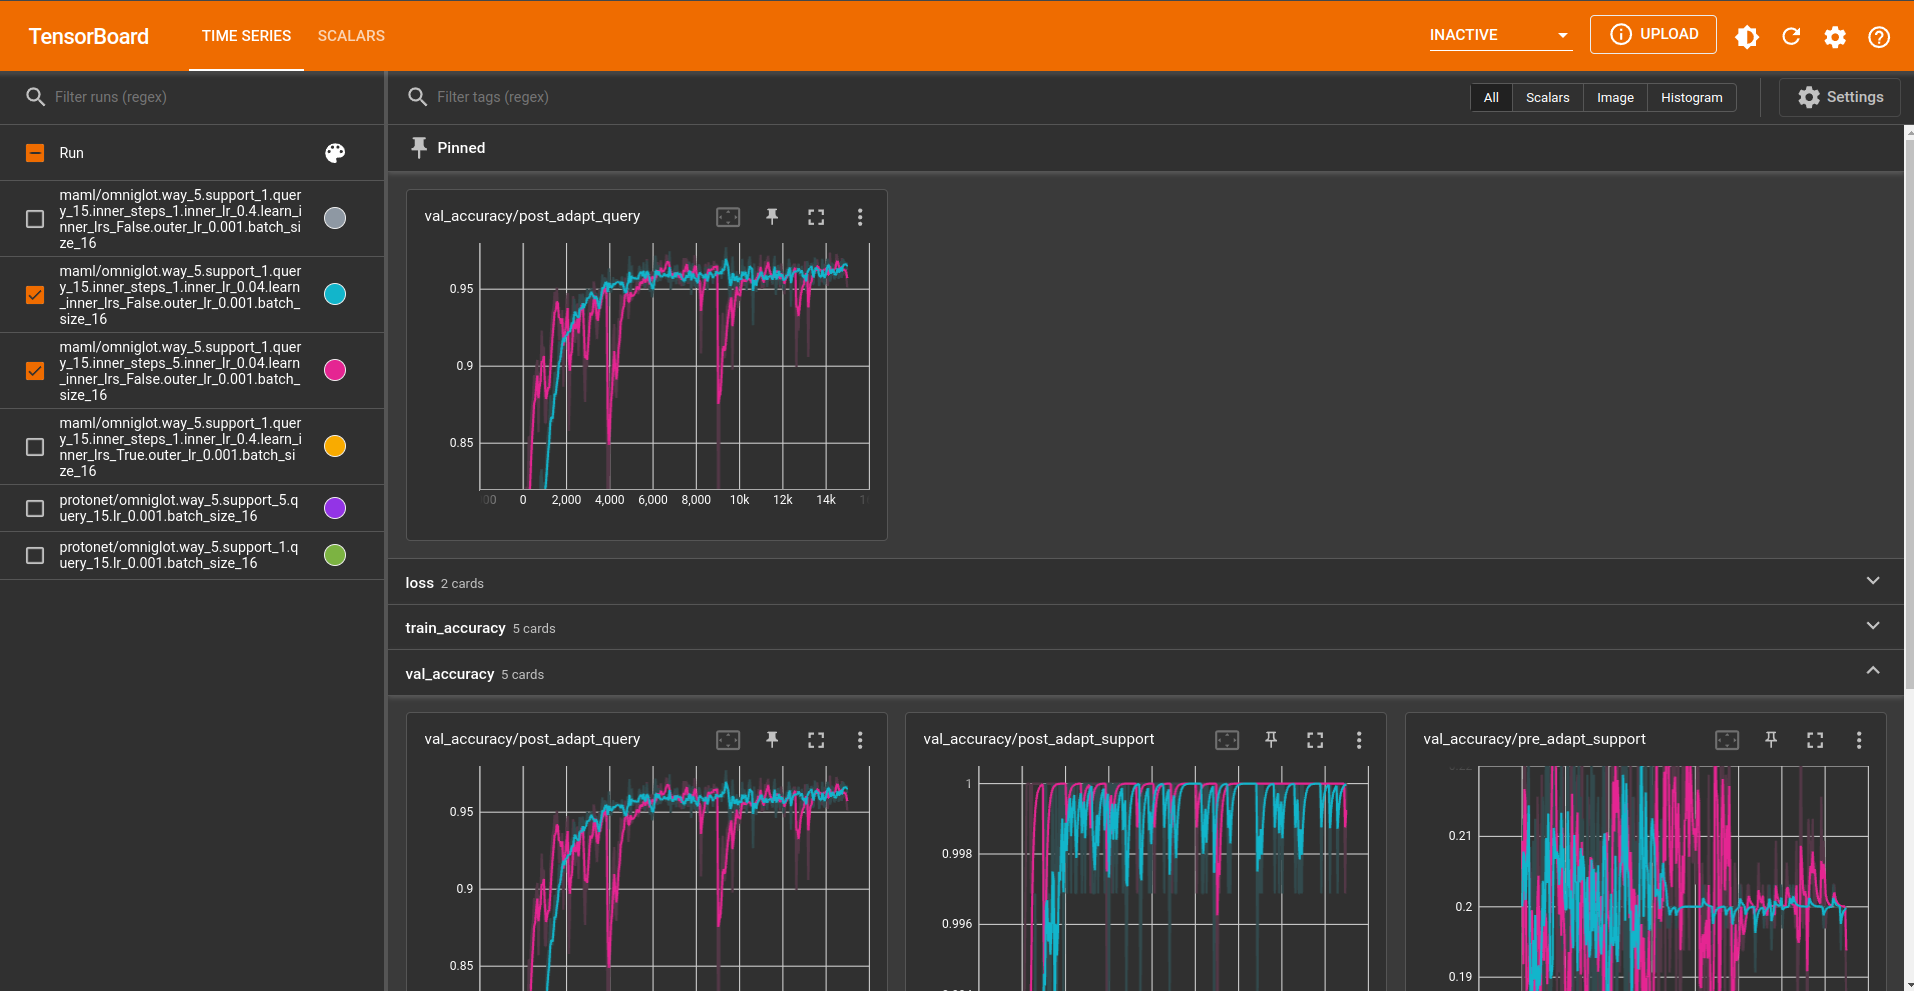
\includegraphics[width=1.0\textwidth]{innerSteps}
	\end{center}
	The effect of increasing the number of inner loop steps is that the model learned faster but took longer to stabilize accuracy. \\
    % ### END CODE HERE ###
\end{answer}
% <SCPD_SUBMISSION_TAG>_2_d_ii

\LARGE
2.d.iii
\normalsize

% <SCPD_SUBMISSION_TAG>_2_d_iii
\begin{answer}
    % ### START CODE HERE ###
	\begin{center}
		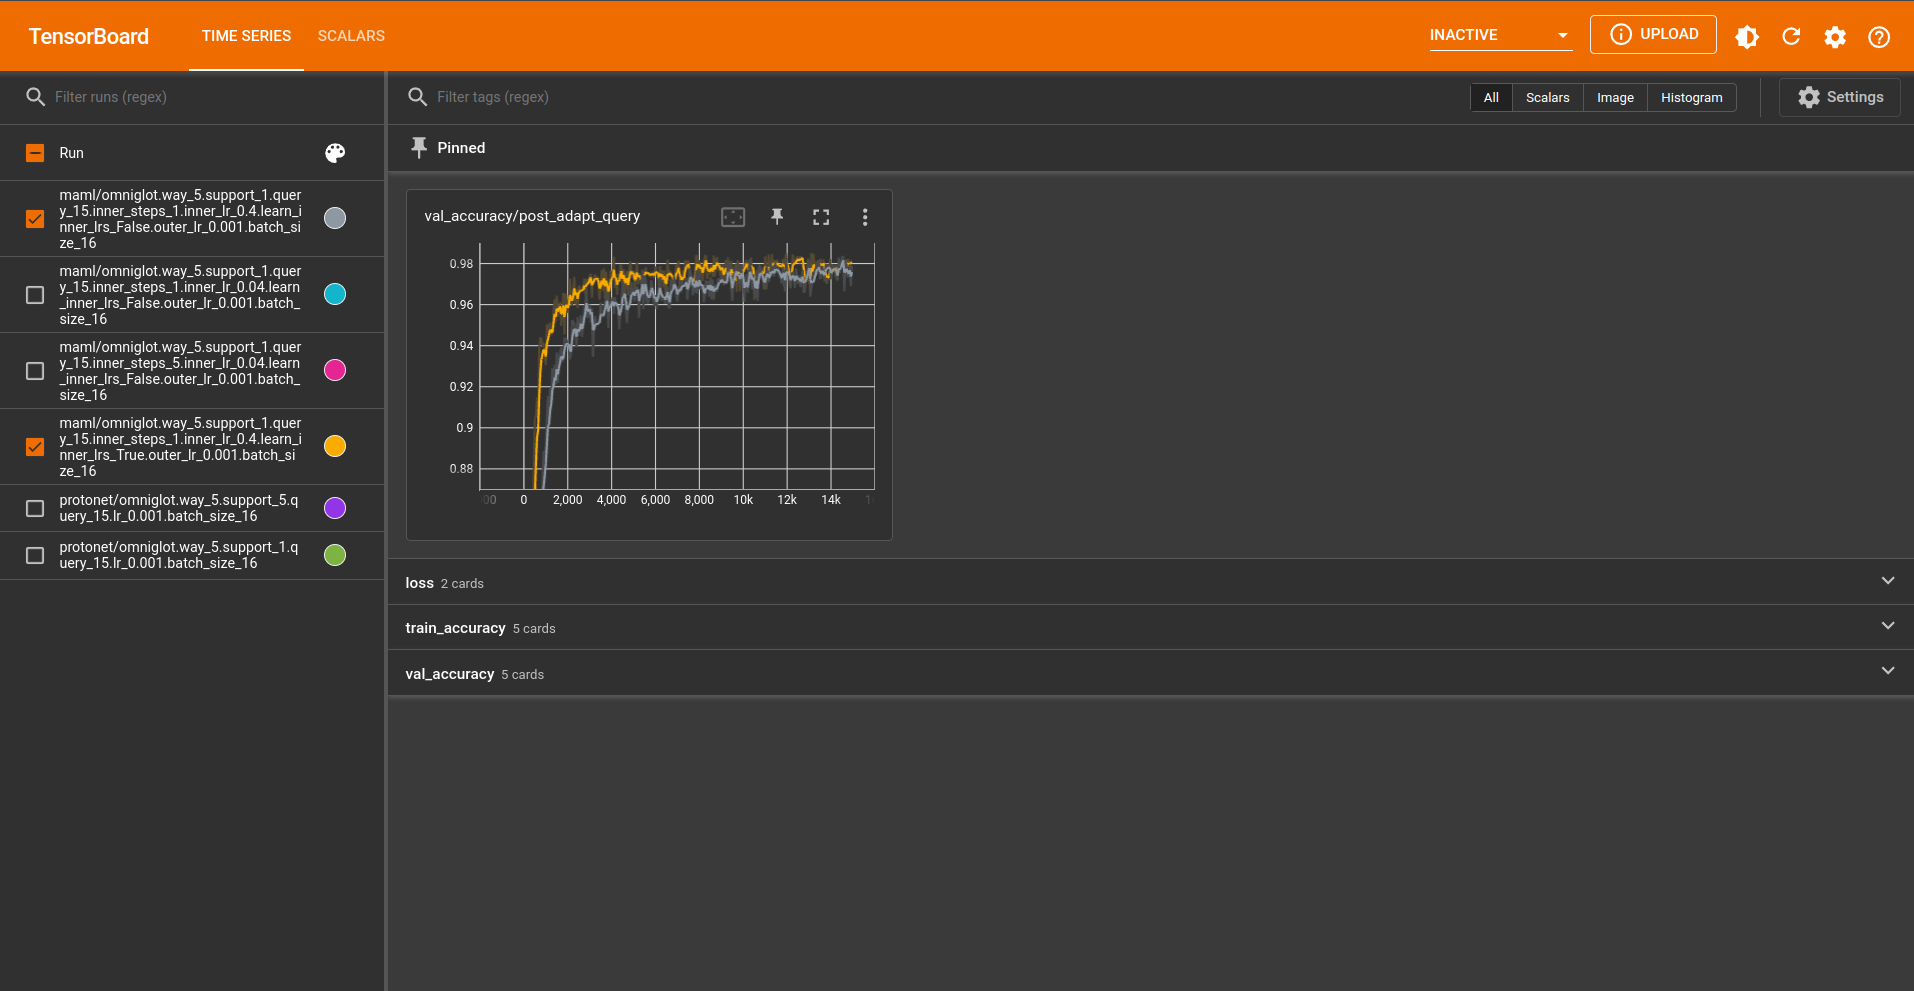
\includegraphics[width=1.0\textwidth]{learnLR}
	\end{center}
	The effect of learning the inner learning rates on optimization is that the model learns faster and remains stable. \\
	This indicates that outer-loop optimization is faster and continues to generalize.
    % ### END CODE HERE ###
\end{answer}
% <SCPD_SUBMISSION_TAG>_2_d_iii


% <SCPD_SUBMISSION_TAG>_entire_submission


\end{document}
